\documentclass[russian]{beamer}

% To be compiled with pdflatex
% (XeTeX's font is somewhat bigger (?), so on some slides the text does not fit into the slide borders)

\usepackage{mystyle}

\graphicspath{ {images/} }

\usetheme{Warsaw} % Warsaw Copenhagen Madrid CambridgeUs Darmstadt Frankfurt Singapore
\setbeamertemplate{headline}{}

\definecolor{beamer@blendedblue}{RGB}{0, 83, 83}  % 104
\definecolor{my-red}{RGB}{176, 0, 0}
\definecolor{my-blue}{RGB}{0, 0, 153}


% Inserting frame numbers in footline
% http://tex.stackexchange.com/questions/191198/customization-of-the-copenhagen-theme
\makeatletter
  \iffalse
  \pgfdeclarehorizontalshading[frametitle.bg,frametitle right.bg]{beamer@frametitleshade}{\paperheight}{%
    color(0pt)=(myblue2);
    color(\paperwidth)=(white)}
  \fi

  \defbeamertemplate*{footline}{mysplit theme}
  {%
    \leavevmode%
    \hbox{\begin{beamercolorbox}[wd=.5\paperwidth,ht=2.5ex,dp=1.125ex,leftskip=.3cm plus1fill,rightskip=.3cm]{author in head/foot}%
      \usebeamerfont{author in head/foot}\insertshortauthor
    \end{beamercolorbox}%
    \begin{beamercolorbox}[wd=.5\paperwidth,ht=2.5ex,dp=1.125ex,leftskip=.3cm,rightskip=.3cm plus1fil]{title in head/foot}%
      \usebeamerfont{title in head/foot}\insertshorttitle\hfill
      \insertframenumber\ / \inserttotalframenumber\hspace*{0.5em}
    \end{beamercolorbox}}%
    \vskip0pt%
  }
\makeatother


\setbeamertemplate{navigation symbols}{} % switch off navigation bar
\setbeamertemplate{itemize item}[ball] % Загадка, но без этого у itemize не будет кружочков
\setbeamertemplate{itemize subitem}[triangle]


% https://tex.stackexchange.com/questions/12735/can-one-replace-bullet-points-with-graphics
\newcommand{\labelitemi}{\usebeamertemplate{itemize item}{}}
\newcommand{\labelitemii}{\usebeamertemplate{itemize subitem}{}}


\AtBeginSection[]
{
  \begin{frame}
    \frametitle{Содержание}
    \tableofcontents[currentsection]
  \end{frame}
}


% https://tex.stackexchange.com/questions/530518/reset-footnote-counter-for-each-frame-in-beamer-class
\AtBeginEnvironment{frame}{\setcounter{footnote}{0}}


\title[Advanced Python 2]
{Введение в анализ данных\\
{\normalsize (Что по чём)}}
\subtitle{}

\author[Василий А.]{
  Алексеев Василий
}

\institute[]
{
  %\textsuperscript{$\diamondsuit$}%
  МФТИ
}

\date[2023]
{
  \footnotesize{1 февраля 2023}
}

\begin{document}

  \frame{\titlepage}
  
  \begin{frame}{План}
    \begin{figure}
      \centering
      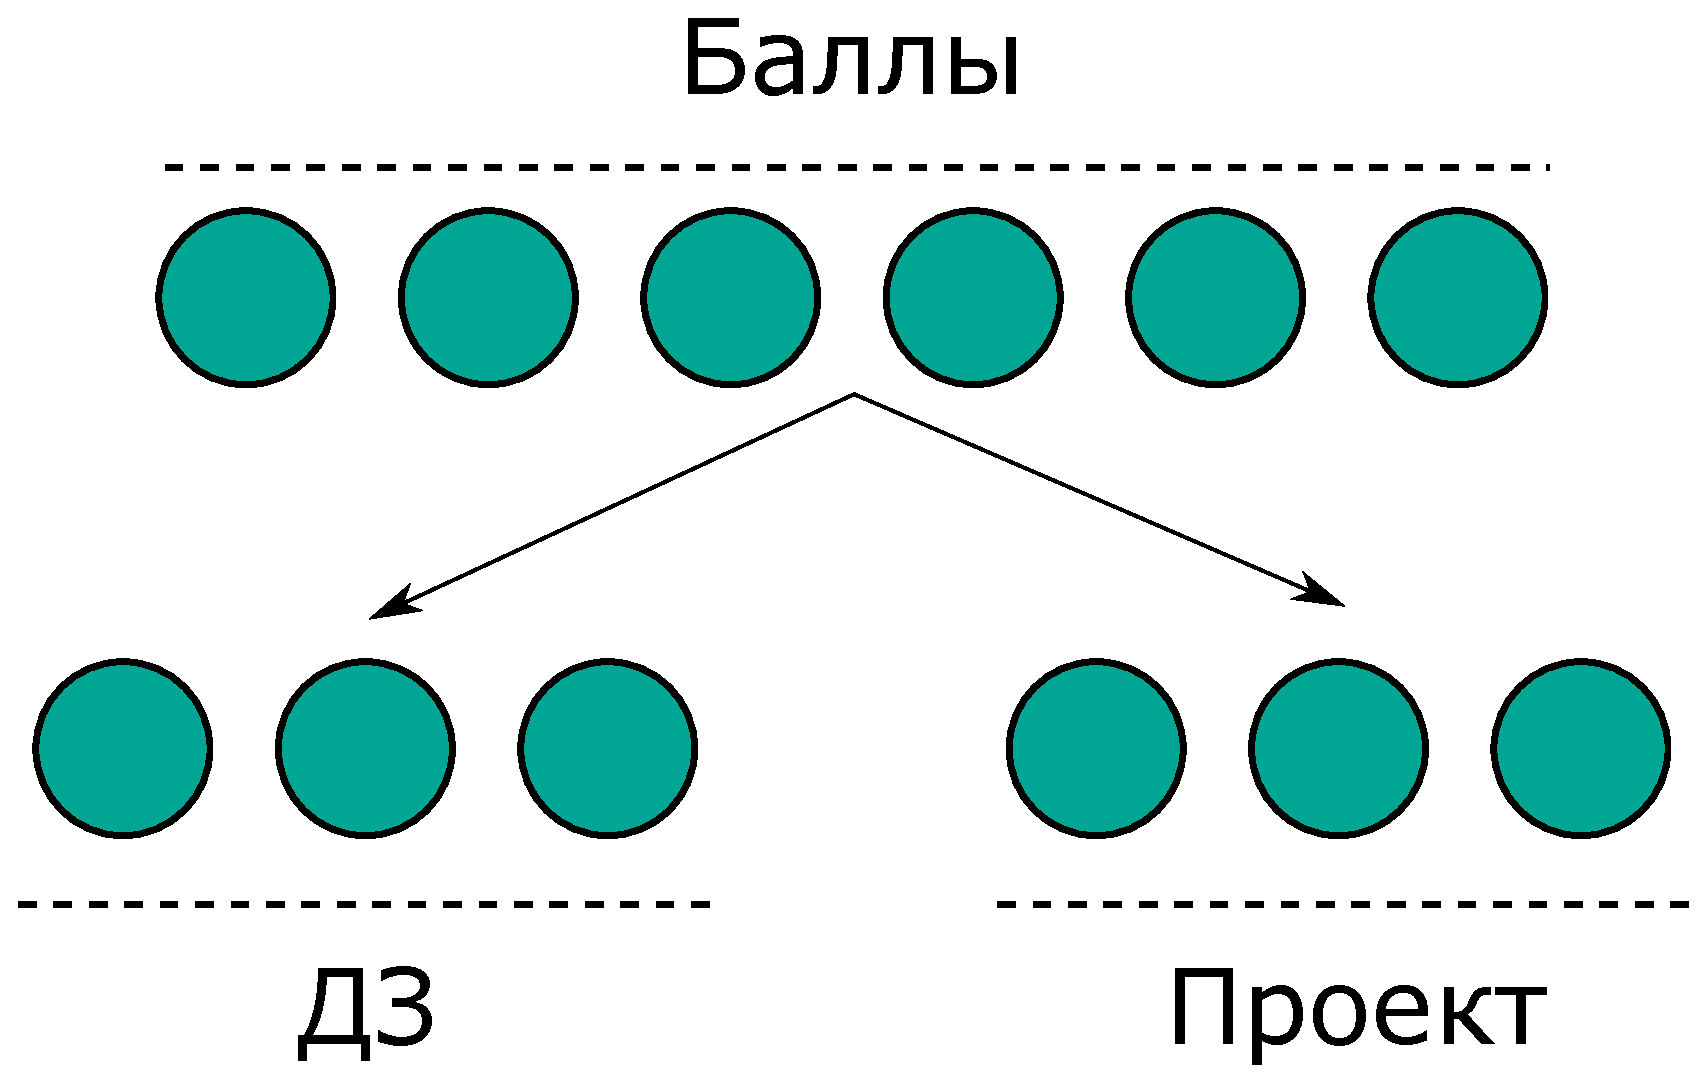
\includegraphics[width=0.75\textwidth]{scheme}
    \end{figure}
  \end{frame}
  
  \begin{frame}{ДЗ}
  
    \pause
    
    Количество $\approx 7$.
    
    \pause
  
    \begin{itemize}
      \item Матрицы (\texttt{numpy})
        \pause
      \item Таблицы (\texttt{pandas})
        \pause
      \item Графики (\texttt{matplotlib})
        \pause
      \item SQL (\texttt{sqlite3})
        \pause
      \item Web (\texttt{flask})
        \pause
      \item ML (\texttt{sklearn})
    \end{itemize}
  \end{frame}
  
  \begin{frame}{Проект}
  
    \pause
    
    Оценивается $6$ пунктов:
    
    \pause
  
    \begin{itemize}
      \item \textbf{``Идея''}: что-то осмысленное.
        \pause
      \item \textbf{Репозиторий}: код, описание.
        \pause
      \item \textbf{Регулярно}: коммиты в течение семестра.
        \pause
      \item \textbf{Командно}: по $\sim$два человека.
        \pause
      \item \textbf{``Анализ данных''}: в каком-то виде.
        \pause
      \item \textbf{Сдача}: в конце семестра.
    \end{itemize}
    
    \pause
    
    \begin{block}{}
      Проект~---~можно как что-то более \emph{исследовательское}, или более \emph{разработческое}.
    \end{block}
  \end{frame}
\end{document}
